\documentclass{article}
\usepackage{bm}
\usepackage{amsmath}
\usepackage{amssymb}
\usepackage{listings}
\usepackage{graphicx}
\usepackage{mdwlist}
\usepackage[colorlinks=true]{hyperref}
\usepackage{geometry}
\geometry{margin=1in}
\geometry{headheight=2in}
\geometry{top=2in}
\usepackage{palatino}
%\renewcommand{\rmdefault}{palatino}
\usepackage{fancyhdr}
%\pagestyle{fancy}
\rhead{}
\lhead{}
\chead{%
  {\vbox{%
      \vspace{2mm}
      \large
      Introduction to Deep Learning M2177.0043 \hfill
\\
      Seoul National University
      \\[4mm]
      Homework \#\textbf{2}\\
      \textbf{Donghak Lee}
    }
  }
}


\usepackage{paralist}

\usepackage{todonotes}
\setlength{\marginparwidth}{2.15cm}

\usepackage{tikz}
\usetikzlibrary{positioning,shapes,backgrounds}

\begin{document}
\pagestyle{fancy}

\section*{INSTRUCTIONS}

\begin{itemize*}
\item Anything
  that is received after the deadline will be considered to be late and we do not receive late homeworks. We do however ignore your lowest homework grade. 
\item Answers to every theory questions need to be submitted
  electronically on ETL. Only PDF generated from LaTex is accepted.
\item Make sure you prepare the answers to each question
  separately. This helps us dispatch the problems to different graders.
\item Collaboration on solving the homework is allowed. Discussions
  are encouraged but you should think about the problems on your own. 
\item If you do collaborate with someone or use a book or website, you
  are expected to write up your solution independently.  That is,
  close the book and all of your notes before starting to write up
  your solution. 
\end{itemize*}

%!TEX root = hw1_2017-12751.tex

%% Q1
\section{Learning a binary classifier with gradient descent}


\subsection {Derive the subgradient of the loss function}
\textbf {Small proof 1.} $g_1, g_2 \in \delta f(x)$ and $a, b$ $(a+b=1, a \geq 0, b\geq 0)$.
\[ a * ( f(y) \geq f(x) + g_1^T(y-x) )\]
\[ b * ( f(y) \geq f(x) + g_2^T(y-x) )\]
\[ \Rightarrow f(y) \geq f(x) + (ag_1 + bg_2)^T(y-x) \]
$\therefore$ Subdifferential is convex set.\\
\textbf{Proof} If $f_1, f_2 : \mathbb{R}^n \rightarrow \mathbb{R}$, convex and differentiable,
\[ Max(f_1(y), f_2(y)) \geq f_1(y) \geq f_1(x) + \nabla f_1(x)^T(y-x) \]
\[ Max(f_1(y), f_2(y)) \geq f_2(y) \geq f_2(x) + \nabla f_2(x)^T(y-x) \]
By \textbf{small proof 1}, $g = a\nabla f_1(x) + b\nabla f_2(x) $ when $(f_1(x) = f_2(x))$
\[\therefore \delta Max(f_1(x), f_2(x)) = \Bigg\{
\begin{tabular}{l r}
$ \nabla f_1(x) $ & $(f_1(x) > f_2(x))$ \\
$ \nabla f_2(x) $ & $(f_1(x) < f_2(x))$ \\
$ a\nabla f_1(x) + b\nabla f_2(x) $ & $(f_1(x) = f_2(x))$
\end{tabular}\]
By \textbf{Proof}, subgradient of $max(0, 1-y_iW^Tx_i)$ is
\[g_i = \bigg\{
\begin{tabular}{l r}
$ 0 $ & $(1 < y_iW^Tx_i)$ \\
$ -\frac{y_i x_i}{n} $ & $(1 \geq y_iW^Tx_i)$ 
\end{tabular}\]
(WLOG, let a = 1, b = 0 to make simple) \\
Because $\frac{\lambda}{2}||W||^2$ is convex and differentiable, its subgradient is $\lambda W$. \\
\textbf{Small proof 2.} If subgradient of $f_i(x) = g_i$, subgradient of $\Sigma{f_i(x)} = \Sigma{g_i}$
\[( \because \Sigma f_i(y) \geq \Sigma (f_i(x) + g_i^T(y-x)) = \Sigma f_i(x) + (\Sigma g_i)^T (y-x) )\]
By \textbf{small proof 2}, subgradient of the loss function is $$\sum_{i=1}^{n}g_i + \lambda W$$

\subsection {}

\lstinputlisting[language=Python]{2_1.py}

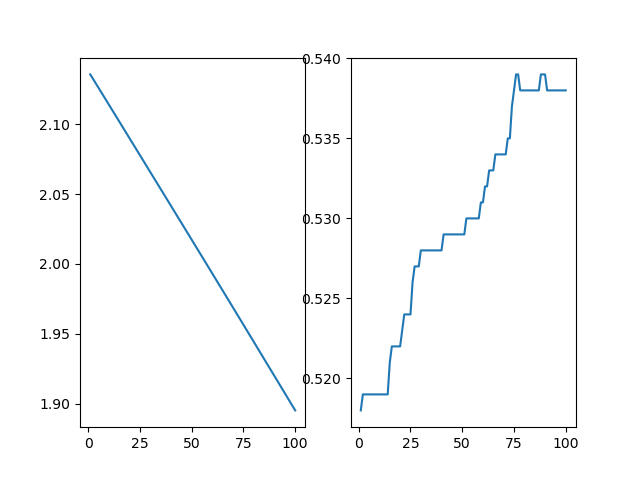
\includegraphics{1-2.png}
	
%% Q2
\section{Matrix estimation with positive semidefinite constraint}

\lstinputlisting[language=Python]{2_2.py}

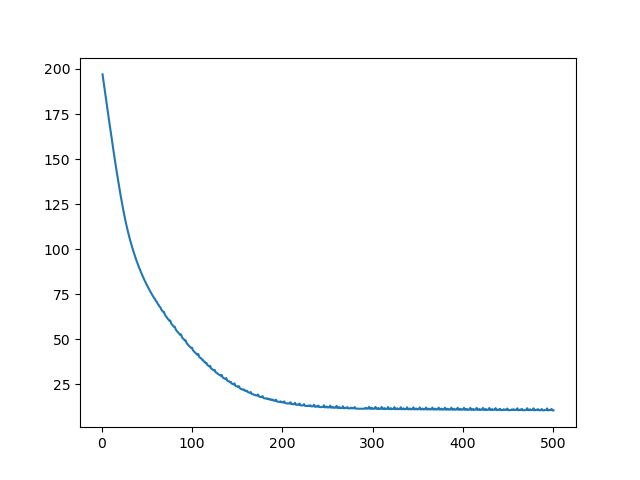
\includegraphics{2-1.png}

\end{document}
